\documentclass[a4paper, 12pt]{article}%тип документа

%отступы
\usepackage[left=2cm,right=2cm,top=2cm,bottom=3cm,bindingoffset=0cm]{geometry}

%Русский язык
\usepackage[T2A]{fontenc} %кодировка
\usepackage[utf8]{inputenc} %кодировка исходного кода
\usepackage[english,russian]{babel} %локализация и переносы

%Вставка картинок
\usepackage{wrapfig}
\usepackage{graphicx}
\graphicspath{{pictures/}}
\DeclareGraphicsExtensions{.pdf,.png,.jpg}

%оглавление
\usepackage{titlesec}
\titlespacing{\chapter}{0pt}{-30pt}{12pt}
\titlespacing{\section}{\parindent}{5mm}{5mm}
\titlespacing{\subsection}{\parindent}{5mm}{5mm}
\usepackage{setspace}

%Графики
\usepackage{multirow}
\usepackage{pgfplots}
\pgfplotsset{compat=1.9}

%Математика
\usepackage{amsmath, amsfonts, amssymb, amsthm, mathtools}

%Стиль страницы
\usepackage{fancyhdr}
\pagestyle{fancy}

\begin{document}

\begin{titlepage}

\begin{center}
%\vspace*{1cm}
\large\textbf{Московский Физико-Технический Институт}\\
\large\textbf{(государственный университет)}
\vfill
\line(1,0){430}\\[1mm]
\huge\textbf{Работа 25}\\
\line(1,0){430}\\[1mm]
\vfill
\large Сибгатуллин Булат, ФРКТ\\
\end{center}

\end{titlepage}
\fancyhead[L] {Работа 25}
\noindent \textbf{Цель работы:} \\
\indent text\\
\noindent \textbf{В работе используются:} \\
\indent text

\section{Выполнение задания}

\subsection{Ознакомительные шаги}

\begin{enumerate}

\item Откроем в Micro-Cap файл adm3p.cir, в котором подготовлены схемы лестничных фильтров порядка \textit{n} = 3, реализующих входной адмиттанс.

\end{enumerate}

%Вставка изображения
%\begin{figure}[h!]
%\centering
%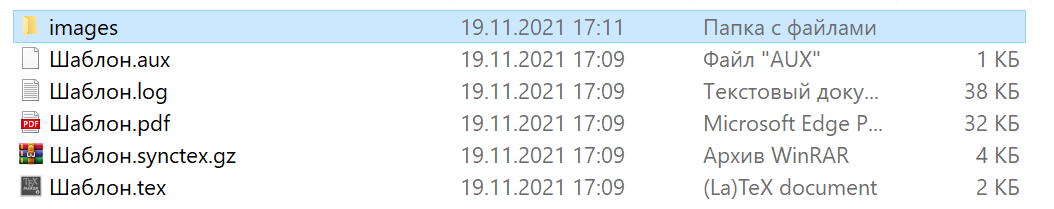
\includegraphics[scale=1]{images/image.png}
%\caption{text}
%\label{fig:Image1}
%\end{figure}

\subsection{Трехполюсные лестничные фильтры}

\begin{enumerate}

\item Откроем модель adm3p.cir и реализуем лестничные фильтры третьего порядка с параметрами:

\[R_0 = 50, \quad f_0 = 1MHz, \quad Q = 10.\]

Для этого вычислим эталонные значения:

\[L_0 = \frac{R_0}{2\pi f_0}, \quad C_0 = \frac{1}{2 \pi f_0 R_0}\]

и установим на схеме номиналы компонентов $f_0, Q, R_0, L_0, C_0$.

\item Сравним частотный характеристики фильтров с теоретическими, удостоверимся в правильности расчетов.

\item Сравним частотные характеристики по напряжению и по мощности. Измерим уровни затухания по мощности на границах полос пропускания, там где затухание по напряжению составляет 0.7. Запишем получившиеся данные в таблицу:

\begin{center}
\begin{tabular}{|c|c|c|c|c|}
\hline 
 & ФНЧ & ФВЧ & Полосовой & Режекторный \\ 
\hline 
Затухание по мощности & 0,5 & 0,5 & 0,5 & 0,5 \\ 
\hline 
\end{tabular} 
\end{center}

Исследуем степень деградации характеристик фильтра нижних частот при варьировании сопротивления источника \textit{RSL} и нагрузки \textit{RLL} от 25 до 75 с шагом 25.

\begin{center}
\begin{tabular}{|c|c|c|c|c|}
\hline 
 & \multicolumn{2}{c|}{RLL} & \multicolumn{2}{c|}{RSL} \\ 
\hline 
 & Напряжение & Мощность & Напряжение & Мощность \\ 
\hline 
25 & 0,33 & 0,44 & 0,66 & 1,77 \\ 
\hline 
50 & 0,5 & 1 & 0,5 & 1 \\ 
\hline 
75 & 0,6 & 1,43 & 0,4 & 0,625 \\ 
\hline 
\end{tabular} 
\end{center}

\item Изучим фазовые характеристики фильтров, измерим значения фазовых сдвигов на нулевой и бесконечной частотах:

\begin{center}
\begin{tabular}{|c|c|c|c|c|}
\hline 
$\omega$ & ФНЧ & ФВЧ & Полосовой & Режекторный \\ 
\hline 
0 & 0 & $-\pi/2$ & $3\pi/2$ & 0 \\ 
\hline 
$\infty$ & $-3\pi/2$ & $-2\pi$ & $-3\pi/2$ & 0 \\ 
\hline 
\end{tabular}
\end{center} 

\item Выведем логарифмическую частотную характеристику фильтра нижних частот в диапазоне $1Meg,100k$ (логарифмическая шкала) и измерим по ней уровни затухания в децибелах на частотах $0, f_0, 2f_0, 10f_0$:

\begin{center}
\begin{tabular}{|c|c|c|c|c|}
\hline 
$f$ & 0 & $f_0$ & $2f_0-$ & $10f_0$ \\ 
\hline 
$K(f_0)$ & -6 & -9 & -24,2 & -66 \\ 
\hline 
\end{tabular} 
\end{center}

\item Выведем логарифмическую частотную характеристику полосового фильтра в диапазоне $1500k,500k$ (линейная шкала) и измерим по ней уровень подавления на частоте $f_0$:

\[K(f_0) = -6 \: dB.\]

Измерим одностороннюю ширину $\bigtriangleup f$ полосы пропускания по уровню $-3 dB$ и уровень затухания при расстройках на $2\bigtriangleup f$, $10\bigtriangleup f$ от частоты $f_0$:

\[\bigtriangleup f = 49\: k\]

\[K(f_0 - 2\bigtriangleup f) = -19 \: dB, \quad K(f_0 + 2\bigtriangleup f) = -16 \: dB\]

\[K(f_0 - 10\bigtriangleup f) = -69,7 \: dB, \quad K(f_0 + 10\bigtriangleup f) = -55 \: dB\]

\item По логарифмической частотной характеристике режекторного фильтра в диапазоне частот $1500,500k$ измерим ширины полос по уровням $-3dB, -43dB, -63dB$:

\begin{center}
\begin{tabular}{|c|c|c|c|}
\hline 
$K(f_0 \pm \bigtriangleup f), \: dB$ & $-3$ & $-43$ & $-63$ \\ 
\hline 
$2\bigtriangleup f$ & 50k & 10k & 4,5k \\ 
\hline 
\end{tabular} 
\end{center}

\end{enumerate}

\section{Фильтры низших частот высших порядков}

\begin{enumerate}

\item Откроем модель batt.cir, в которой реализованы фильтры Баттерворта нижних частот с параметрами $R_0 = 100, f_0 = 1MHz (L_0= 15.916, C_0 = 1.592n)$ порядков от 3 до 7. Изучим их частотные и переходные характеристики. По логарифмическим графикам в диапазоне $10Meg, 100k$ измерим затухания на частотах $f_0, 2f_0$ и $10f_0$:

\begin{center}
\begin{tabular}{|c|c|c|c|c|c|}
\hline 
Фильтр Баттерворта & n=3 & n=4 & n=5 & n=6 & n=7 \\ 
\hline 
$K(f_0), \: dB$ & -3.03 & -3.04 & -3.04 & -3.04 & -3.04 \\ 
\hline 
$K(2f_0), \: dB$ & -18.15 & -24.13 & -30.13 & -36.15 & -42.18 \\ 
\hline 
$K(10f_0), \: dB$ & -60.02 & -80.03 & -100.03 & -120.03 & -140.03 \\ 
\hline 
\end{tabular} 
\end{center}

\item Повторим те же исследования для фильтров Чебышева с неравномерностями 0.5 dB (файл cheb0-5.cir) и 3 dB (файл cheb3-0.cir)

\begin{center}
\begin{tabular}{|c|c|c|c|c|c|}
\hline 
Чебышева 0.5 dB & n=3 & n=4 & n=5 & n=6 & n=7 \\ 
\hline 
$K(f_0), \: dB$ & • & • & • & • & • \\ 
\hline 
$K(2f_0), \: dB$ & • & • & • & • & • \\ 
\hline 
Чебышева 3.0 dB & • & • & • & • & • \\ 
\hline 
$K(f_0), \: dB$ & • & • & • & • & • \\ 
\hline 
$K(2f_0), \: dB$ & • & • & • & • & • \\ 
\hline 
\end{tabular} 
\end{center}

\end{enumerate}

\end{document}